\documentclass[peerreviewca]{IEEEtran}

\usepackage[utf8]{inputenc}
\usepackage[T1]{fontenc}
\usepackage{cite}
\usepackage{amsmath,amssymb,amsfonts}
\usepackage{graphicx}
\usepackage{textcomp}
\usepackage{xcolor}
\usepackage{booktabs}
\usepackage{multirow}
\usepackage{hyperref}

% Figures are read from the repository outputs, so the PDF always uses the committed notebook exports.
\graphicspath{{figures/}{../outputs/maps/}{../outputs/figures/}{../docs/}}

\begin{document}

\title{Mexico City Urban Intelligence: A Geospatial Data Warehouse Integrating Demographic, Economic and Public-Safety Data at Urban AGEB Level}

\author{\IEEEauthorblockN{Ricardo Daniel Horta S\'anchez}
  \IEEEauthorblockA{Data Engineering\\
    Universidad Polit\'ecnica de Yucat\'an\\
    Km. 4.5. Carretera M\'erida --- Tetiz\\
    Tablaje Catastral 4448. CP 97357\\
    Uc\'u, Yucat\'an. M\'exico\\
    Email: 2309122@upy.edu.mx}
  \and
  \IEEEauthorblockN{Jos\'e \'Angel Pech Xool}
  \IEEEauthorblockA{Data Engineering\\
    Universidad Polit\'ecnica de Yucat\'an\\
    Km. 4.5. Carretera M\'erida --- Tetiz\\
    Tablaje Catastral 4448. CP 97357\\
    Uc\'u, Yucat\'an. M\'exico\\
    Email: 2309175@upy.edu.mx}
  \and
  \IEEEauthorblockN{Valeria Nicol Hern\'andez Le\'on}
  \IEEEauthorblockA{Data Engineering\\
    Universidad Polit\'ecnica de Yucat\'an\\
    Km. 4.5. Carretera M\'erida --- Tetiz\\
    Tablaje Catastral 4448. CP 97357\\
    Uc\'u, Yucat\'an. M\'exico\\
    Email: 2309114@upy.edu.mx}
  \and
  \IEEEauthorblockN{Lorena Danae P\'erez L\'opez}
  \IEEEauthorblockA{Data Engineering\\
    Universidad Polit\'ecnica de Yucat\'an\\
    Km. 4.5. Carretera M\'erida --- Tetiz\\
    Tablaje Catastral 4448. CP 97357\\
    Uc\'u, Yucat\'an. M\'exico\\
    Email: 2309179@upy.edu.mx}
  \and
  \IEEEauthorblockN{Julio C\'esar de Aquino Castellanos}
  \IEEEauthorblockA{Data Engineering\\
    Universidad Polit\'ecnica de Yucat\'an\\
    Km. 4.5. Carretera M\'erida --- Tetiz\\
    Tablaje Catastral 4448. CP 97357\\
    Uc\'u, Yucat\'an. M\'exico\\
    Email: 2309066@upy.edu.mx}
  \and
  \IEEEauthorblockN{Gustavo Alexander Fuentes Mar\'in}
  \IEEEauthorblockA{Data Engineering\\
    Universidad Polit\'ecnica de Yucat\'an\\
    Km. 4.5. Carretera M\'erida --- Tetiz\\
    Tablaje Catastral 4448. CP 97357\\
    Uc\'u, Yucat\'an. M\'exico\\
    Email: 2309089@upy.edu.mx}
  \and
  \IEEEauthorblockN{Didier Omar Gamboa Angulo}
  \IEEEauthorblockA{Universidad Polit\'ecnica de Yucat\'an\\
    Km. 4.5. Carretera M\'erida --- Tetiz\\
    Tablaje Catastral 4448. CP 97357\\
    Uc\'u, Yucat\'an. M\'exico\\
    Email: didier.gamboa@upy.edu.mx}}

\maketitle

\begin{abstract}
We built a reproducible PostgreSQL/PostGIS data warehouse that integrates the INEGI Population and Housing Census 2020, the INEGI business directory (DENUE 05/2026), the INEGI 2020 geostatistical framework and georeferenced investigation files from the Mexico City Attorney General's Office (FGJ, offences of January--July 2024). The common unit is the urban AGEB: 2,431 polygons covering 792.15~km\textsuperscript{2} and 9,138,524 residents. Point-in-polygon assignment retains 99.7\% of establishments and 93.8\% of eligible crime records. A star schema with three fact tables at their finest grain feeds analytical views from which every KPI and spatial statistic is computed. The three central alcaldías hold 15.3\% of residents but 28.1\% of recorded investigation files, although the gap almost disappears when crime is measured per establishment. Business density, population density, economically active population rate and crime rate are all positively spatially autocorrelated (Moran's $I$ between 0.18 and 0.51). Business and crime hot spots overlap in 35 AGEBs, 31 of them in Cuauht\'emoc. These results are spatial associations, not causal effects.
\end{abstract}

\begin{IEEEkeywords}
Geospatial data warehouse, PostGIS, urban AGEB, spatial autocorrelation, LISA, bivariate Moran's I, Mexico City, crime, DENUE, Census 2020.
\end{IEEEkeywords}

\vspace*{\fill}
    \noindent
\begin{minipage}[c]{0.4\textwidth}
    \centering
    
\includegraphics[width=6cm]{upy-logo}
\end{minipage}
\hspace{1cm}
\begin{minipage}[c]{0.5\textwidth}
    \centering
    
\includegraphics[width=8cm]{gobierno-logo}
\end{minipage}
\vspace{1.5in}
%
% Do not change this
\IEEEpeerreviewmaketitle

\section{Problem and Data Sources}

Residential population, economic activity and recorded crime describe different uses of urban space, and the official sources that measure them do not share a geographic representation. The Census publishes tables keyed by area identifiers, while DENUE and FGJ publish individual records with latitude and longitude. The project integrates the four layers in a single warehouse so that territorial KPIs can be computed, areas compared, and spatial association between layers tested. The study area moved from M\'erida to Mexico City (CDMX) when the only crime data available for M\'erida turned out to be municipal totals, which cannot be assigned to areas within the city. No incidents were simulated.

\begin{table}[htbp]
\caption{Sources and grain}
\label{tab:sources}
\centering
\begin{tabular}{@{}llll@{}}
\toprule
Layer & Source & Grain & Date \\
\midrule
Demographic & Census 2020 \cite{inegi_census} & AGEB totals & Mar 2020 \\
Economic & DENUE \cite{inegi_denue} & establishment & May 2026 \\
Geographic & Marco Geo.\ 2020 \cite{inegi_mg} & AGEB polygon & 2020 \\
Public safety & FGJ files \cite{fgj} & file (point) & Jan--Jul 2024 \\
\bottomrule
\end{tabular}
\end{table}

Table~\ref{tab:sources} lists the sources. INEGI suppresses small Census values (\texttt{*}) and marks some as unavailable (\texttt{N/D}). Both are stored as NULL, never as zero. The FGJ extract contains files opened from 1~January to 31~July 2024, so August--December are unavailable and are not treated as months with zero crime. Every raw file is pinned by a SHA-256 hash in a download manifest.

\section{Geographic Integration Strategy}

We evaluated the alcald\'ia, locality, colonia, a hexagonal grid and the urban AGEB as candidate units. Alcald\'ias (16) hide neighbourhood-scale variation. Localities are few and uneven in size. Colonias are not an INEGI statistical geography, and a hexagonal grid has no Census identifier, so Census counts would have to be interpolated. The urban AGEB is the only unit for which the Census publishes totals and INEGI publishes matching polygons with the same \texttt{CVEGEO} key. All 2,431 polygons have a Census row and valid geometry. Two Census AGEBs without a 2020 polygon (7,108 residents) are dropped and counted. Analyses that need a contiguous area use the 2,348 AGEBs of the main locality of each alcald\'ia (the city core).

All geometries are stored in EPSG:6372 (Mexico ITRF2008 / LCC, metres), the projection of the INEGI cartography, so areas and densities are computed without reprojection. DENUE and FGJ coordinates (EPSG:4326) are projected and assigned with a strict \texttt{within} predicate. Points outside every polygon are counted, never snapped to the nearest one. Table~\ref{tab:join} shows the result. The 1,501 unassigned establishments lie outside the urban AGEB frame (three outside CDMX). The assigned AGEB agrees with the code DENUE reports for 99.84\% of establishments.

\begin{table}[htbp]
\caption{Point-in-polygon assignment}
\label{tab:join}
\centering
\begin{tabular}{@{}lrrr@{}}
\toprule
Source & Input & Assigned & Captured \\
\midrule
DENUE 05/2026 & 462,732 & 461,231 & 99.7\% \\
FGJ 2024 (criminal) & 119,666 & 112,285 & 93.8\% \\
\bottomrule
\end{tabular}
\end{table}

\section{Data Warehouse Architecture}

The pipeline follows RAW $\rightarrow$ CLEAN $\rightarrow$ SPATIAL JOIN $\rightarrow$ PostgreSQL/PostGIS and runs with a single command. One Python module per source cleans the data to a fixed column contract. A shared spatial module assigns points to AGEBs. The cleaned files are written to a staging schema, and SQL scripts resolve surrogate keys into the dimensional schema. The run ends with a validation script that aborts on any failed check. It checks row counts against staging, polygon validity and the 792.15~km\textsuperscript{2} total area, the 9,138,524 Census population, that every point lies inside its assigned AGEB, and that the KPI views reconcile with the fact tables.

Fig.~\ref{fig:model} shows the star schema. The three fact tables keep the finest available grain: one urban AGEB for the Census (2,431 rows), one establishment for DENUE (461,231 rows) and one investigation file for crime (112,285 rows). Establishments and incidents keep their point geometry. They share conformed dimensions for geography (AGEB polygon, alcald\'ia, area), date and source, plus SCIAN activity, business size, crime type and hour. Because aggregation happens only in views, every KPI can be recomputed or re-aggregated without returning to the raw files. \texttt{dim\_source} stores the publisher, URL, original grain and hash of each file, and every fact row references it.

\begin{figure*}[!t]
\centerline{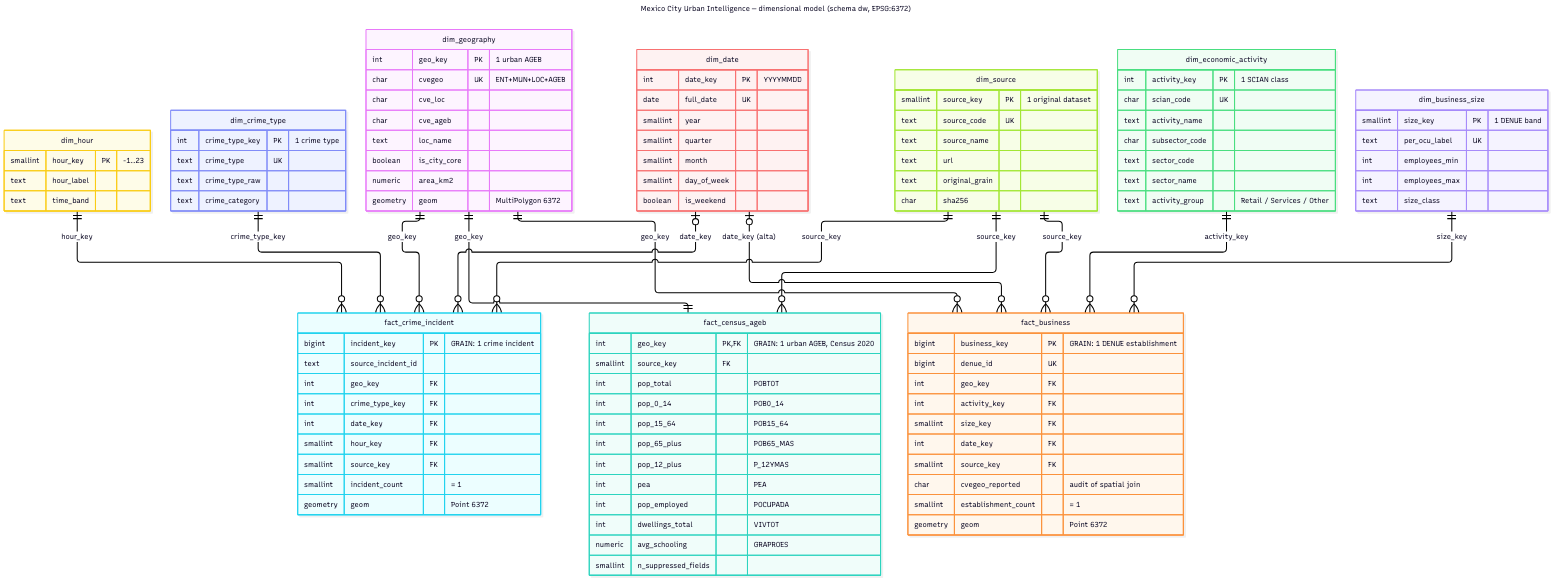
\includegraphics[width=\textwidth]{warehouse_model.png}}
\caption{Dimensional model: three fact tables at their finest grain sharing conformed dimensions (schema \texttt{dw}, EPSG:6372).}
\label{fig:model}
\end{figure*}

\section{Key KPIs and Spatial Analysis}

The view \texttt{v\_kpi\_ageb} returns one row per AGEB with its polygon and the territorial KPIs required by the brief. Demographic KPIs are total population, population density, the economically active population (PEA) rate and age groups. Economic KPIs are total businesses, business, retail and service density, businesses per 1,000 residents and the dominant sector. Public-safety KPIs are total incidents, crime rate per 1,000 residents and crimes per 100 businesses. \texttt{v\_crime\_by\_type\_time} gives the distribution of incidents by type, month, weekday and time band. Every ratio uses \texttt{NULLIF} on its denominator. Alcald\'ia figures are computed as sums of numerators over sums of denominators, not as averages of AGEB ratios. Per-resident rates exclude the 51 city-core AGEBs with fewer than 100 residents, whose ratios are unstable. Fig.~\ref{fig:kpis} maps six KPIs.

\begin{figure*}[!t]
\centerline{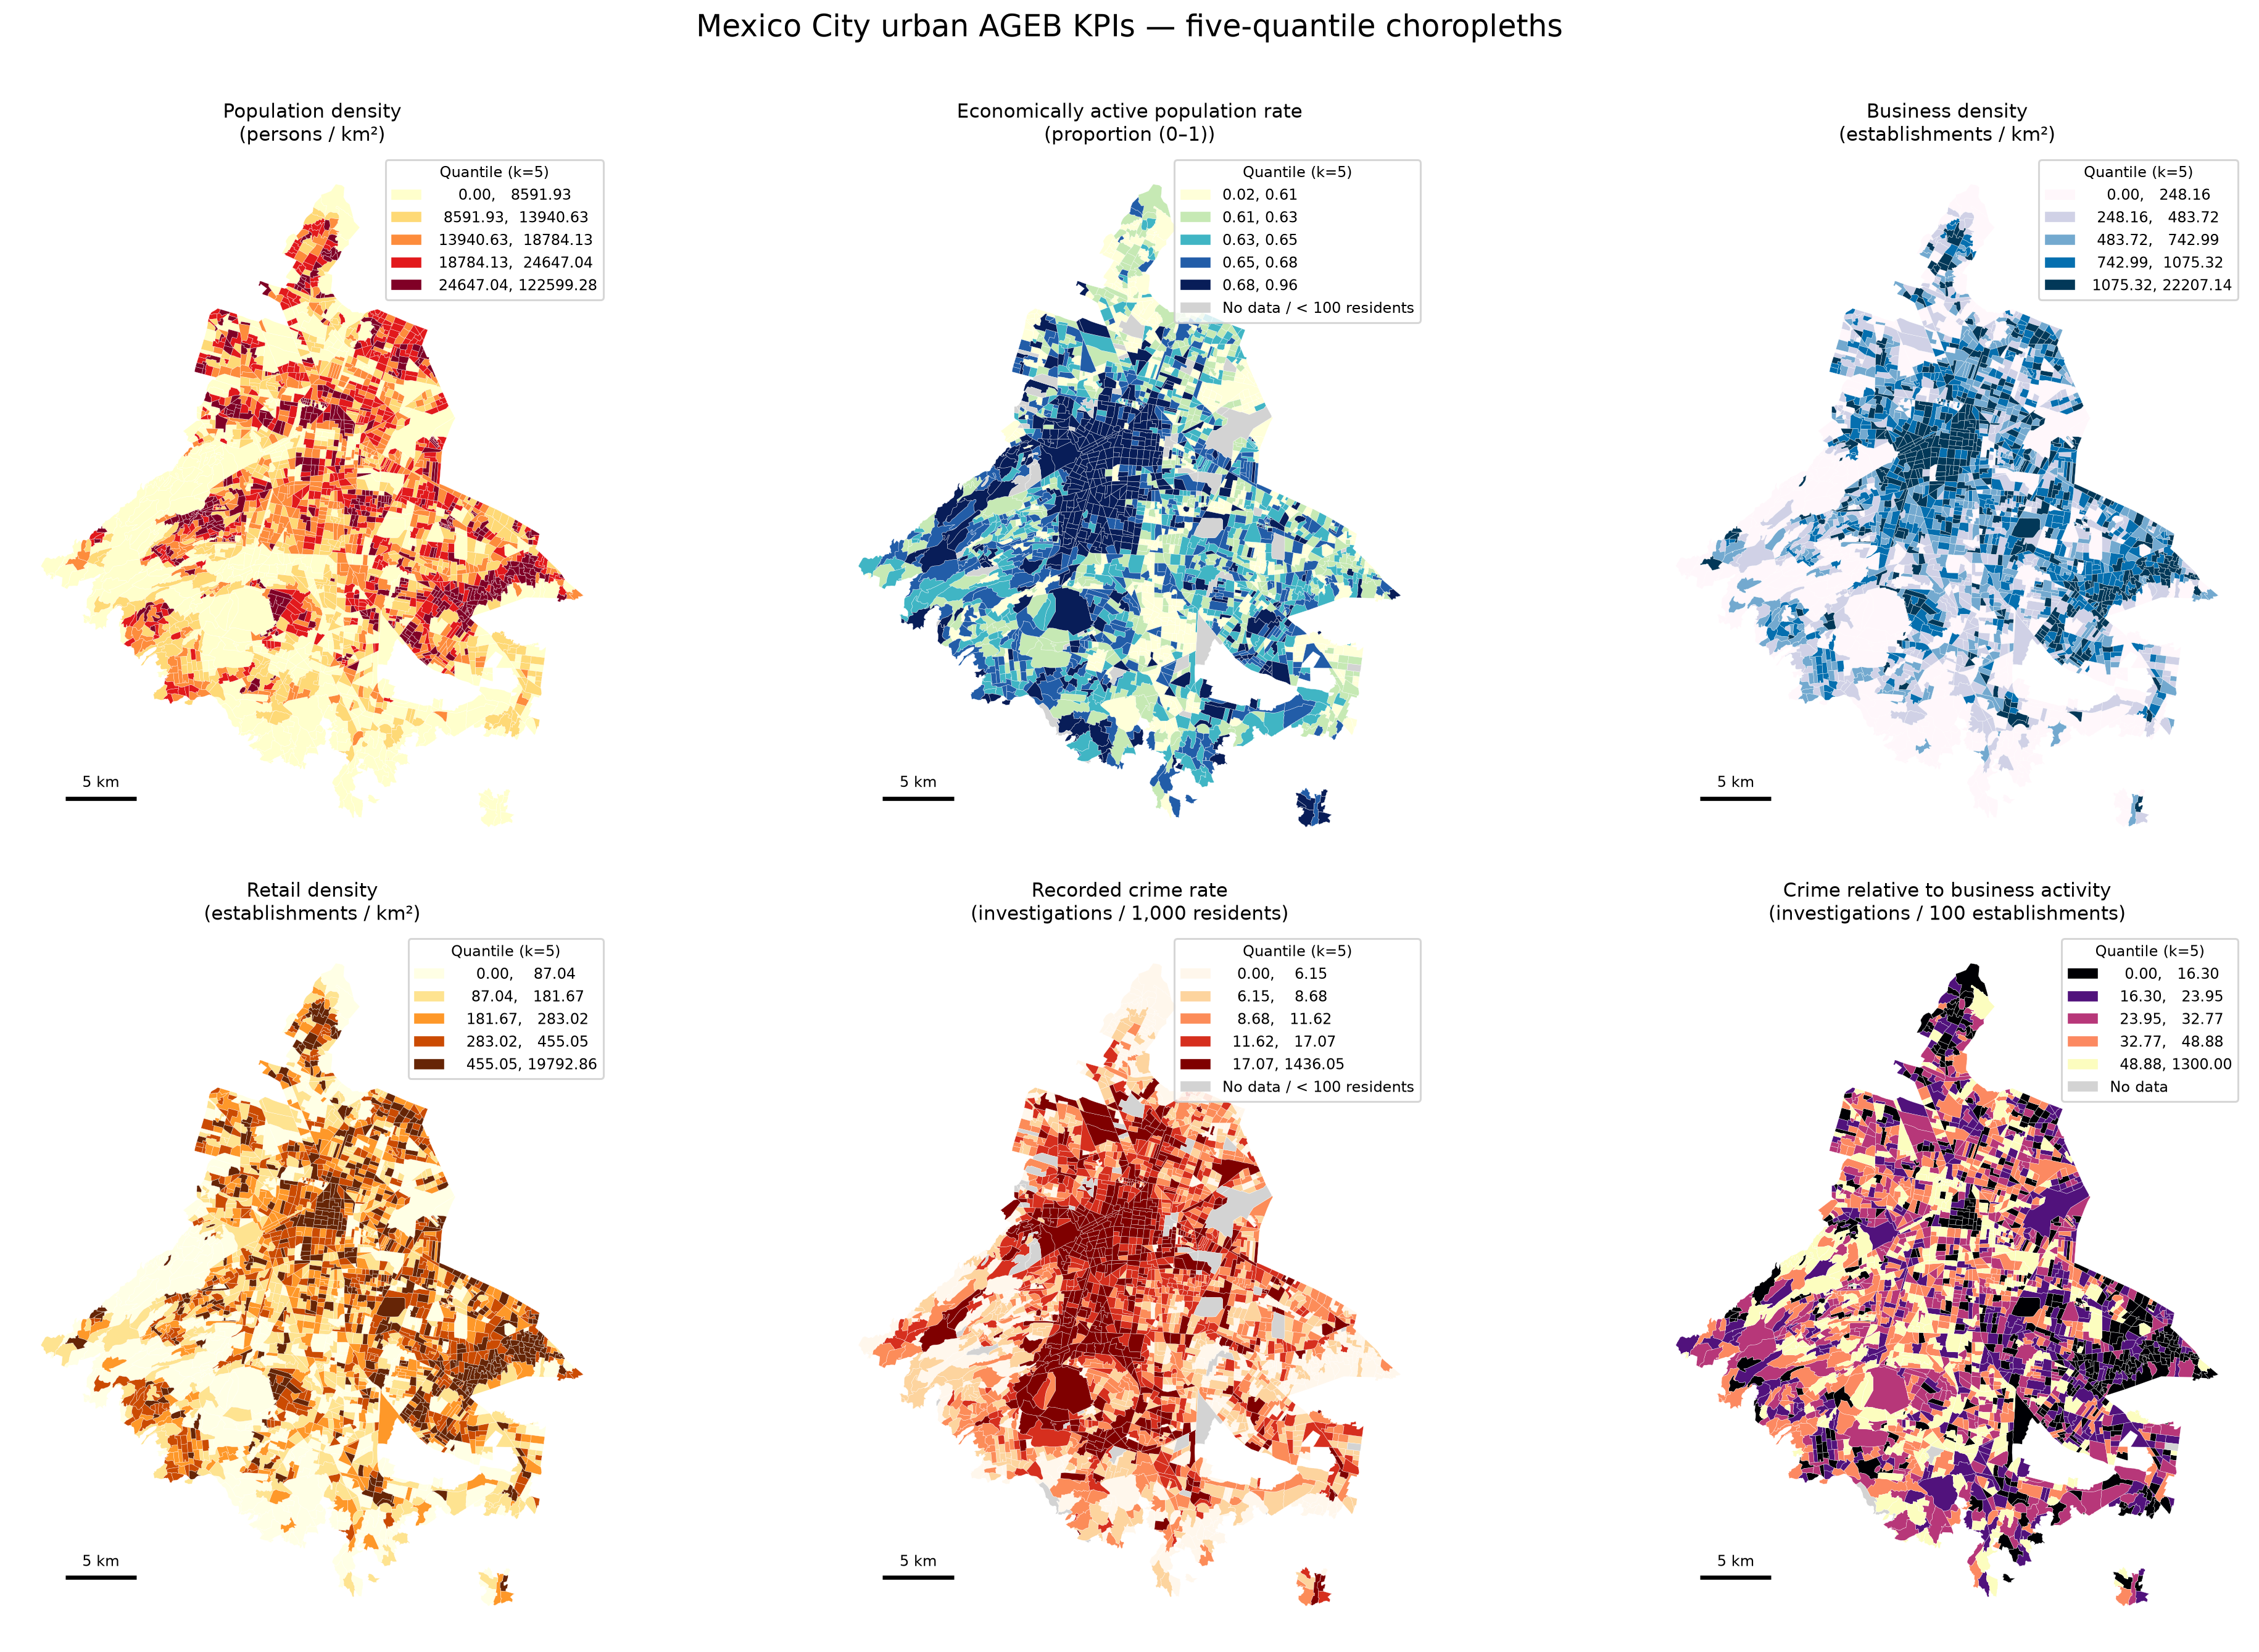
\includegraphics[width=\textwidth]{kpi_choropleths_summary.png}}
\caption{Six KPIs on the 2,348 city-core AGEBs (five-quantile classes). Grey in the per-resident rates marks AGEBs with fewer than 100 residents or an undefined ratio.}
\label{fig:kpis}
\end{figure*}

\textbf{Neighbourhood rule.} The primary spatial weights are row-standardised Queen contiguity on the city core. AGEBs that share a vertex or an edge are neighbours, and the single island is attached to its nearest AGEB. K-nearest neighbours ($k=6$) is the sensitivity rule. Queen weights follow the irregular AGEB geometry, so small central AGEBs have several neighbours within a short distance while large peripheral AGEBs reach further away. KNN-6 gives every AGEB the same number of neighbours. All permutation tests use 999 permutations and seed 42 \cite{rey2007pysal}.

\textbf{Correlation.} All variables reject normality and have heavy right tails, so Spearman's $\rho$ is the primary measure and Pearson's $r$ is reported for comparison (Table~\ref{tab:corr}). The p-values assume independent observations and are not corrected for spatial dependence.

\begin{table}[htbp]
\caption{Correlations, city core, AGEBs with at least 100 residents ($n=2{,}297$)}
\label{tab:corr}
\centering
\begin{tabular}{@{}lrr@{}}
\toprule
Pair & Spearman $\rho$ & Pearson $r$ \\
\midrule
Pop.\ density vs business density & 0.358 & 0.099 \\
Crime rate vs businesses per 1k & 0.580 & 0.794 \\
PEA rate vs crime rate & 0.190 & 0.209 \\
\bottomrule
\multicolumn{3}{@{}p{0.95\columnwidth}@{}}{\footnotesize All $p < 10^{-5}$. With low-population AGEBs: $\rho = 0.378$, $0.589$, $0.179$.}
\end{tabular}
\end{table}

\textbf{Global and local Moran's I.} Table~\ref{tab:moran} shows positive and significant global autocorrelation \cite{moran1950} for the four indicators tested, with similar values under both rules. Local Moran (LISA) \cite{anselin1995} at $\alpha = 0.05$ labels 482 of 2,348 AGEBs for business density (109 High-High, 312 Low-Low, 61 spatial outliers) and 540 of 2,297 for crime rate (110 High-High, 344 Low-Low, 86 outliers). Each AGEB is a separate test, so the labels are exploratory. Under a Benjamini--Hochberg screen \cite{benjamini1995}, 25 business and 12 crime High-High AGEBs remain.

\begin{table}[htbp]
\caption{Global Moran's I (999 permutations, all pseudo $p = 0.001$)}
\label{tab:moran}
\centering
\begin{tabular}{@{}lrrr@{}}
\toprule
Indicator & $n$ & $I$ (Queen) & $I$ (KNN-6) \\
\midrule
Business density & 2,348 & 0.462 & 0.458 \\
Population density & 2,348 & 0.434 & 0.451 \\
PEA rate & 2,297 & 0.506 & 0.500 \\
Crime rate per 1k residents & 2,297 & 0.210 & 0.179 \\
\bottomrule
\end{tabular}
\end{table}

\textbf{Bivariate Moran's I.} Business density in each AGEB is compared with the spatial lag of the crime rate in neighbouring AGEBs. The result is $I = 0.201$ with Queen and $0.207$ with KNN-6 weights (pseudo $p = 0.001$, $n = 2{,}297$). The association persists after a log1p transformation (0.179 and 0.183).

\section{Main Findings}

\textbf{1. The centre concentrates establishments and recorded crime.} Cuauht\'emoc, Benito Ju\'arez and Miguel Hidalgo hold 15.3\% of the urban population, 25.4\% of establishments and 28.1\% of investigation files (Fig.~\ref{fig:alcaldia}). Their crime rate is 22.6 files per 1,000 residents, against 10.4 in the other 13 alcald\'ias. Cuauht\'emoc has 2,089 establishments per km\textsuperscript{2}, more than twice the second alcald\'ia. Iztapalapa, the most populous alcald\'ia (1.84 million residents), has the lowest crime rate (8.4).

\begin{figure*}[!t]
\centerline{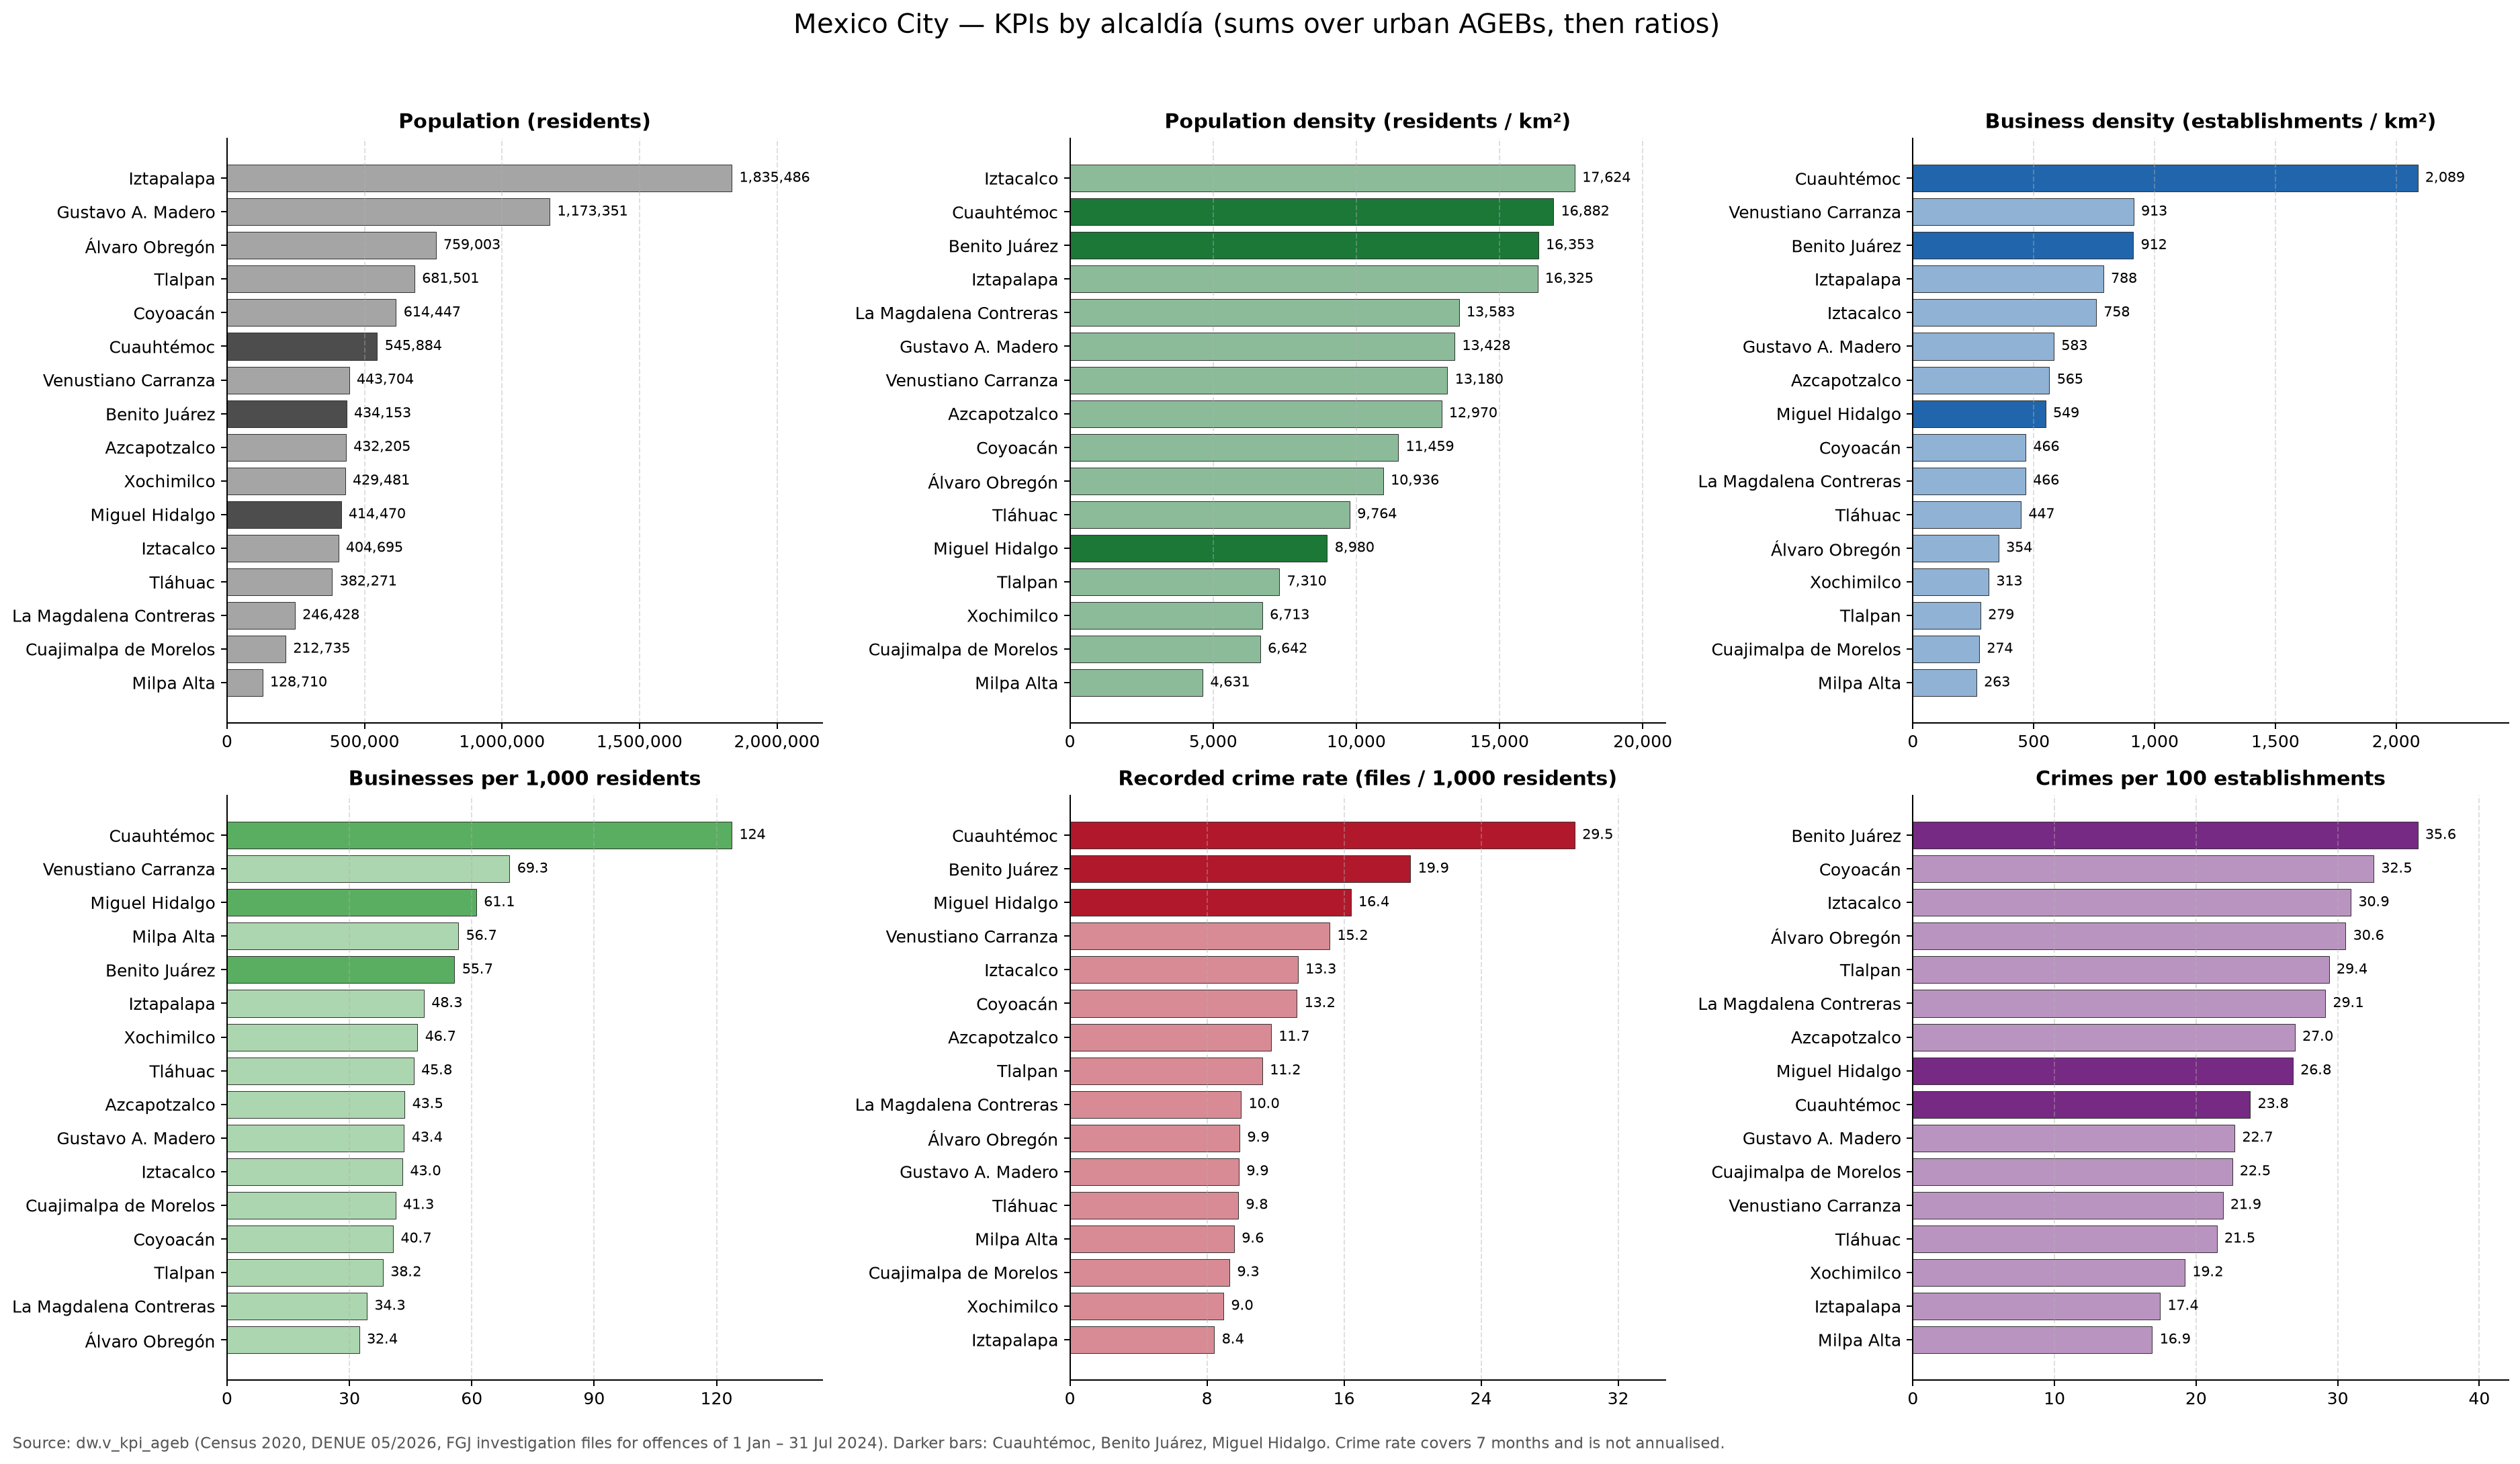
\includegraphics[width=\textwidth]{35_alcaldia_comparison.png}}
\caption{KPIs by alcald\'ia, computed as sums over urban AGEBs and then ratios. Darker bars mark the three central alcald\'ias.}
\label{fig:alcaldia}
\end{figure*}

\textbf{2. The ranking depends on the denominator.} Per establishment, the centre and the rest of the city are close (26.9 vs 23.5 crimes per 100 establishments), and Cuauht\'emoc falls to 9th place. Commuters and visitors are not counted as residents, so per-resident rates overstate resident exposure in the centre. The same mechanism inflates the AGEB-level Pearson coefficient between crime rate and businesses per 1,000 residents ($r = 0.794$ vs $\rho = 0.580$). Both rates divide by the same resident population, which induces correlation between ratios \cite{pearson1897}.

\textbf{3. Business and crime hot spots overlap only partly.} 76 of the 109 business-density hot spots (70\%) are in Cuauht\'emoc. Crime-rate hot spots are more spread out: Cuauht\'emoc has 47 of 110, and the rest are mainly in Miguel Hidalgo, Benito Ju\'arez, Gustavo A. Madero and Venustiano Carranza (Fig.~\ref{fig:lisa}). 35 AGEBs are hot spots for both indicators, 31 of them in Cuauht\'emoc. The largest crime cold spot is in Iztapalapa (164 Low-Low AGEBs). Business hot spots are stable under KNN-6 (88\% remain High-High). Crime hot spots are less stable (59\%).

\begin{figure*}[!t]
\centerline{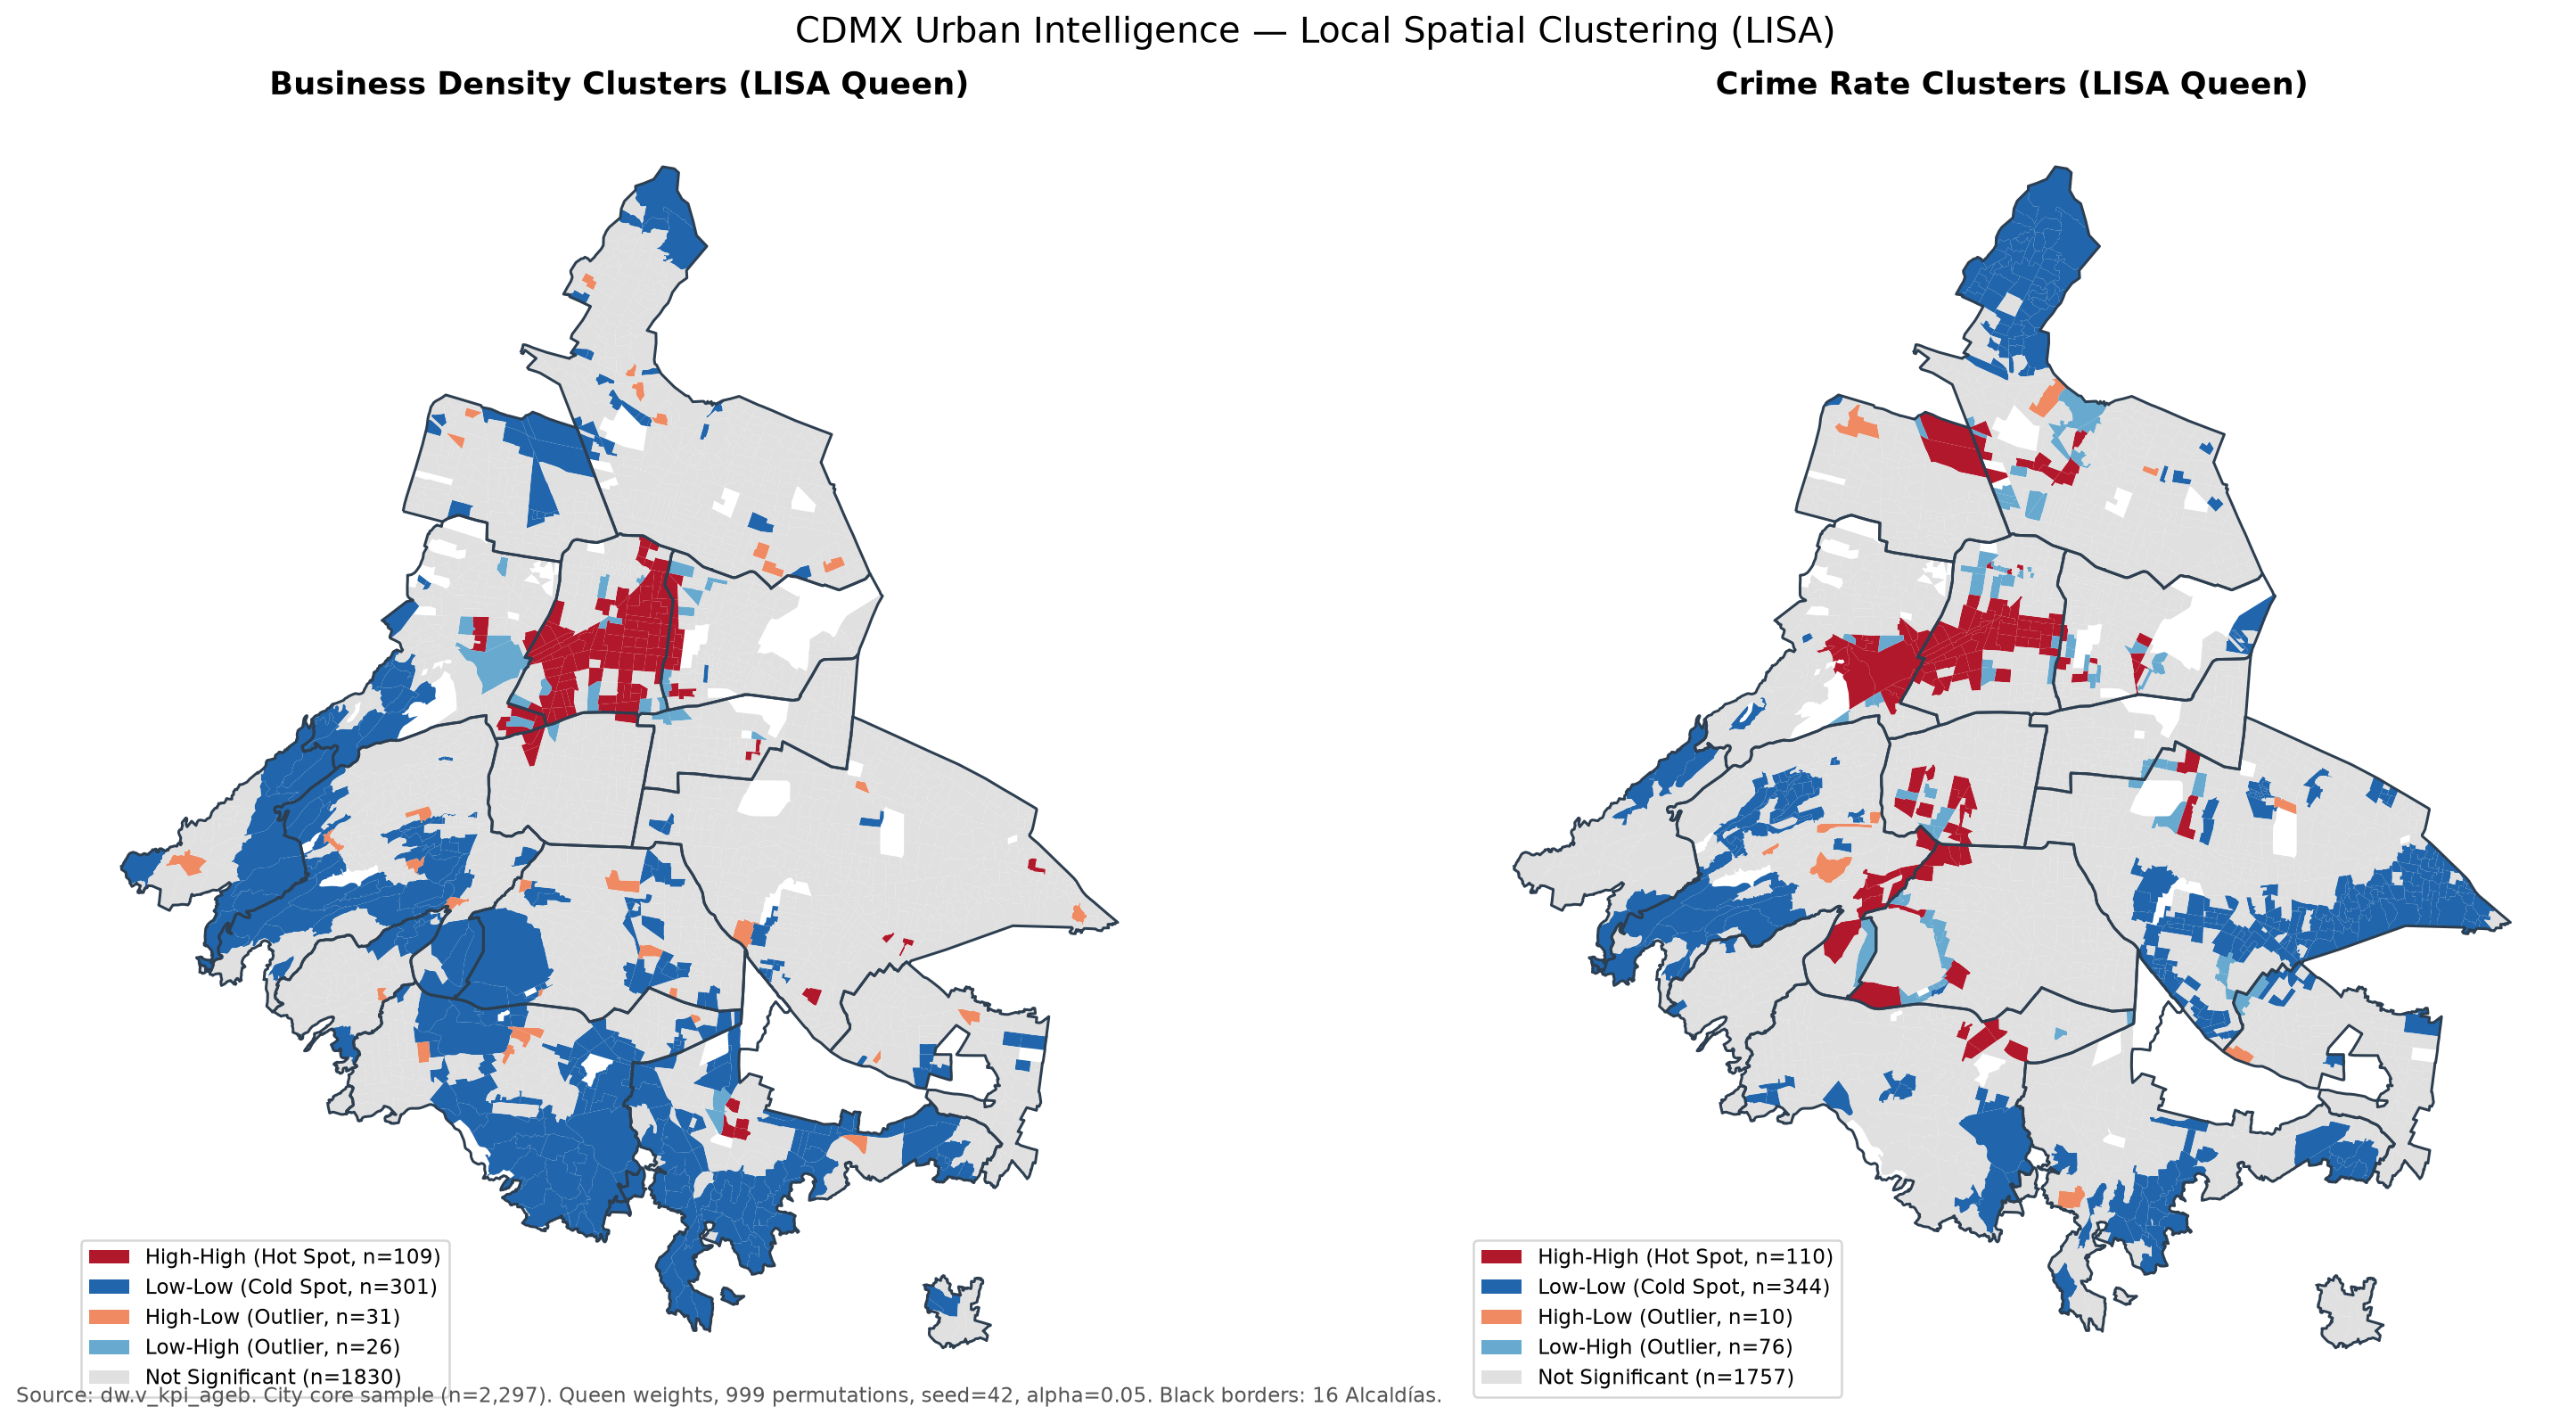
\includegraphics[width=\textwidth]{34_hotspot_clusters_alcaldia.png}}
\caption{LISA clusters of business density and crime rate (Queen, $p<0.05$) and their overlap. Dark outlines are the 16 alcald\'ias.}
\label{fig:lisa}
\end{figure*}

\textbf{4. Business density is associated with neighbouring crime rates.} The bivariate Moran's $I$ of 0.20 is positive and stable under both neighbourhood rules and the log transformation (Fig.~\ref{fig:bv}). AGEBs with more establishments tend to be surrounded by AGEBs with higher recorded crime rates.

\begin{figure}[!tb]
\centerline{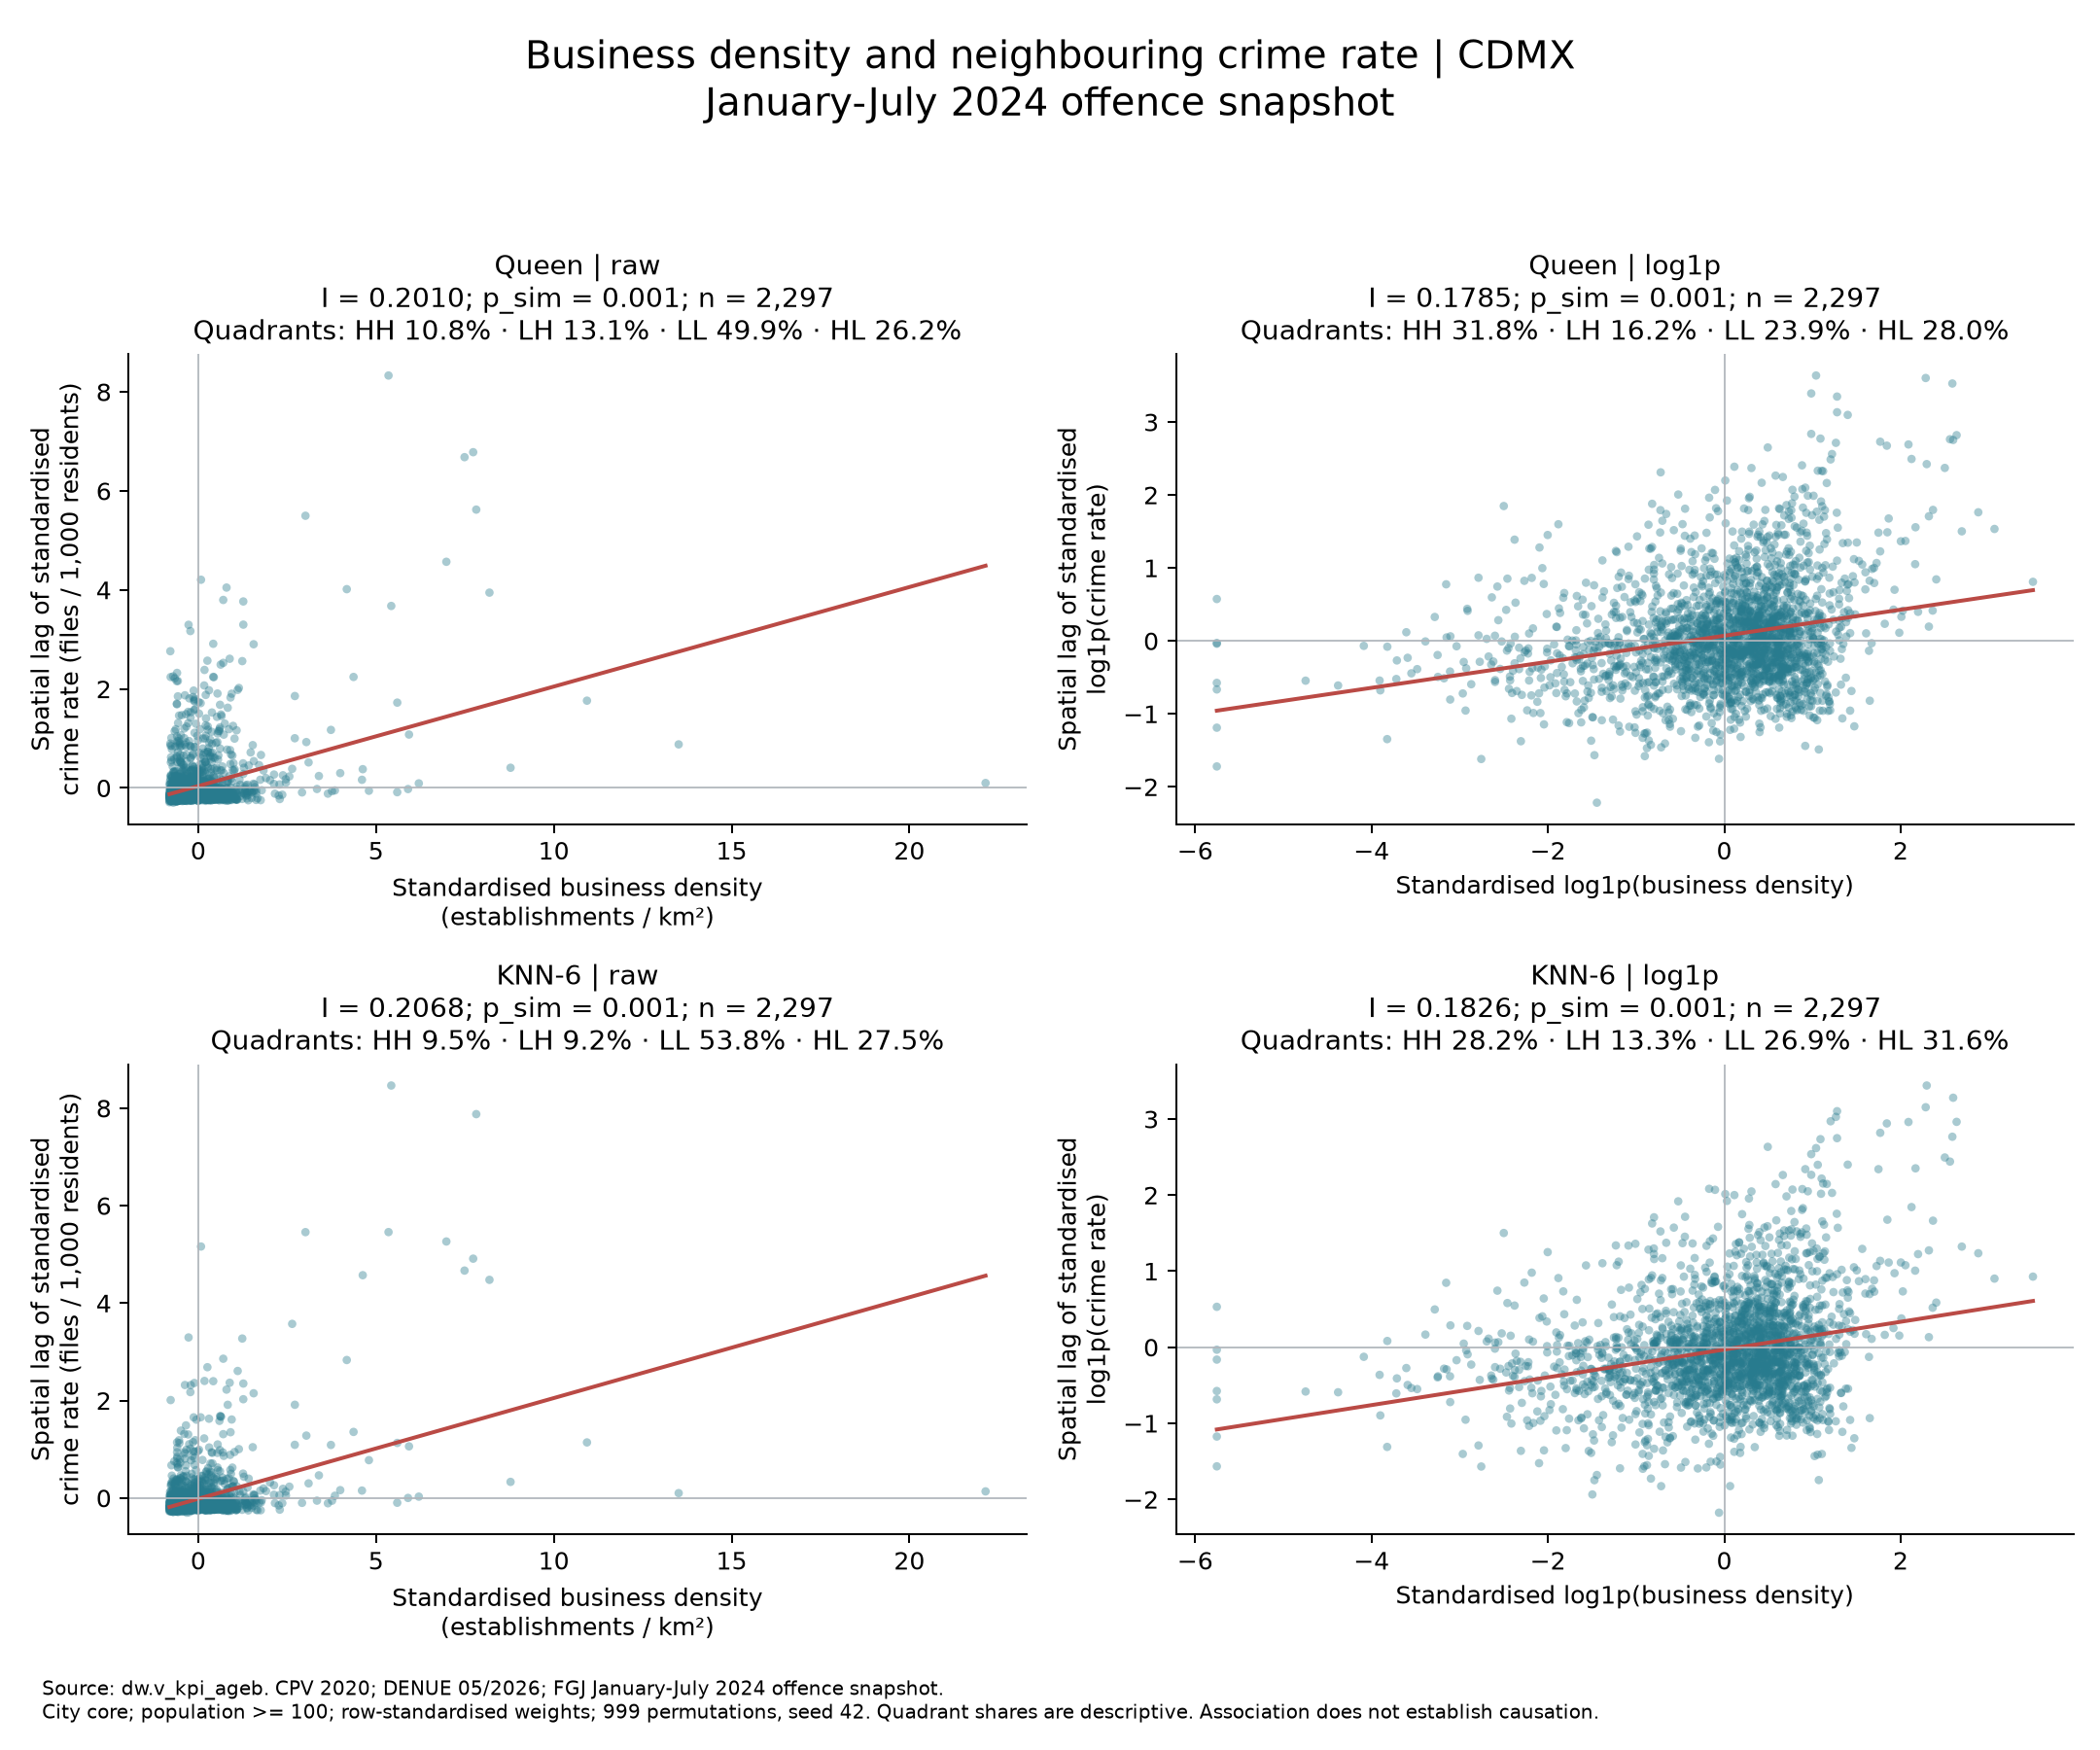
\includegraphics[width=\columnwidth]{bivariate_moran_business_crime.png}}
\caption{Standardised business density against the spatial lag of the standardised crime rate, Queen and KNN-6 weights, raw and log1p scales ($n=2{,}297$).}
\label{fig:bv}
\end{figure}

\textbf{5. Recorded crime peaks in the afternoon and on Fridays.} The afternoon band (12:00--17:59) has 33.7\% of investigation files and the night band 13.2\% (Fig.~\ref{fig:time}). Friday has the highest calendar-adjusted daily average in January--July (567.3) and in the January--June sensitivity that excludes the right-censored July (585.6). Family violence is the most frequent offence type (18.0\%).

\begin{figure}[!tb]
\centerline{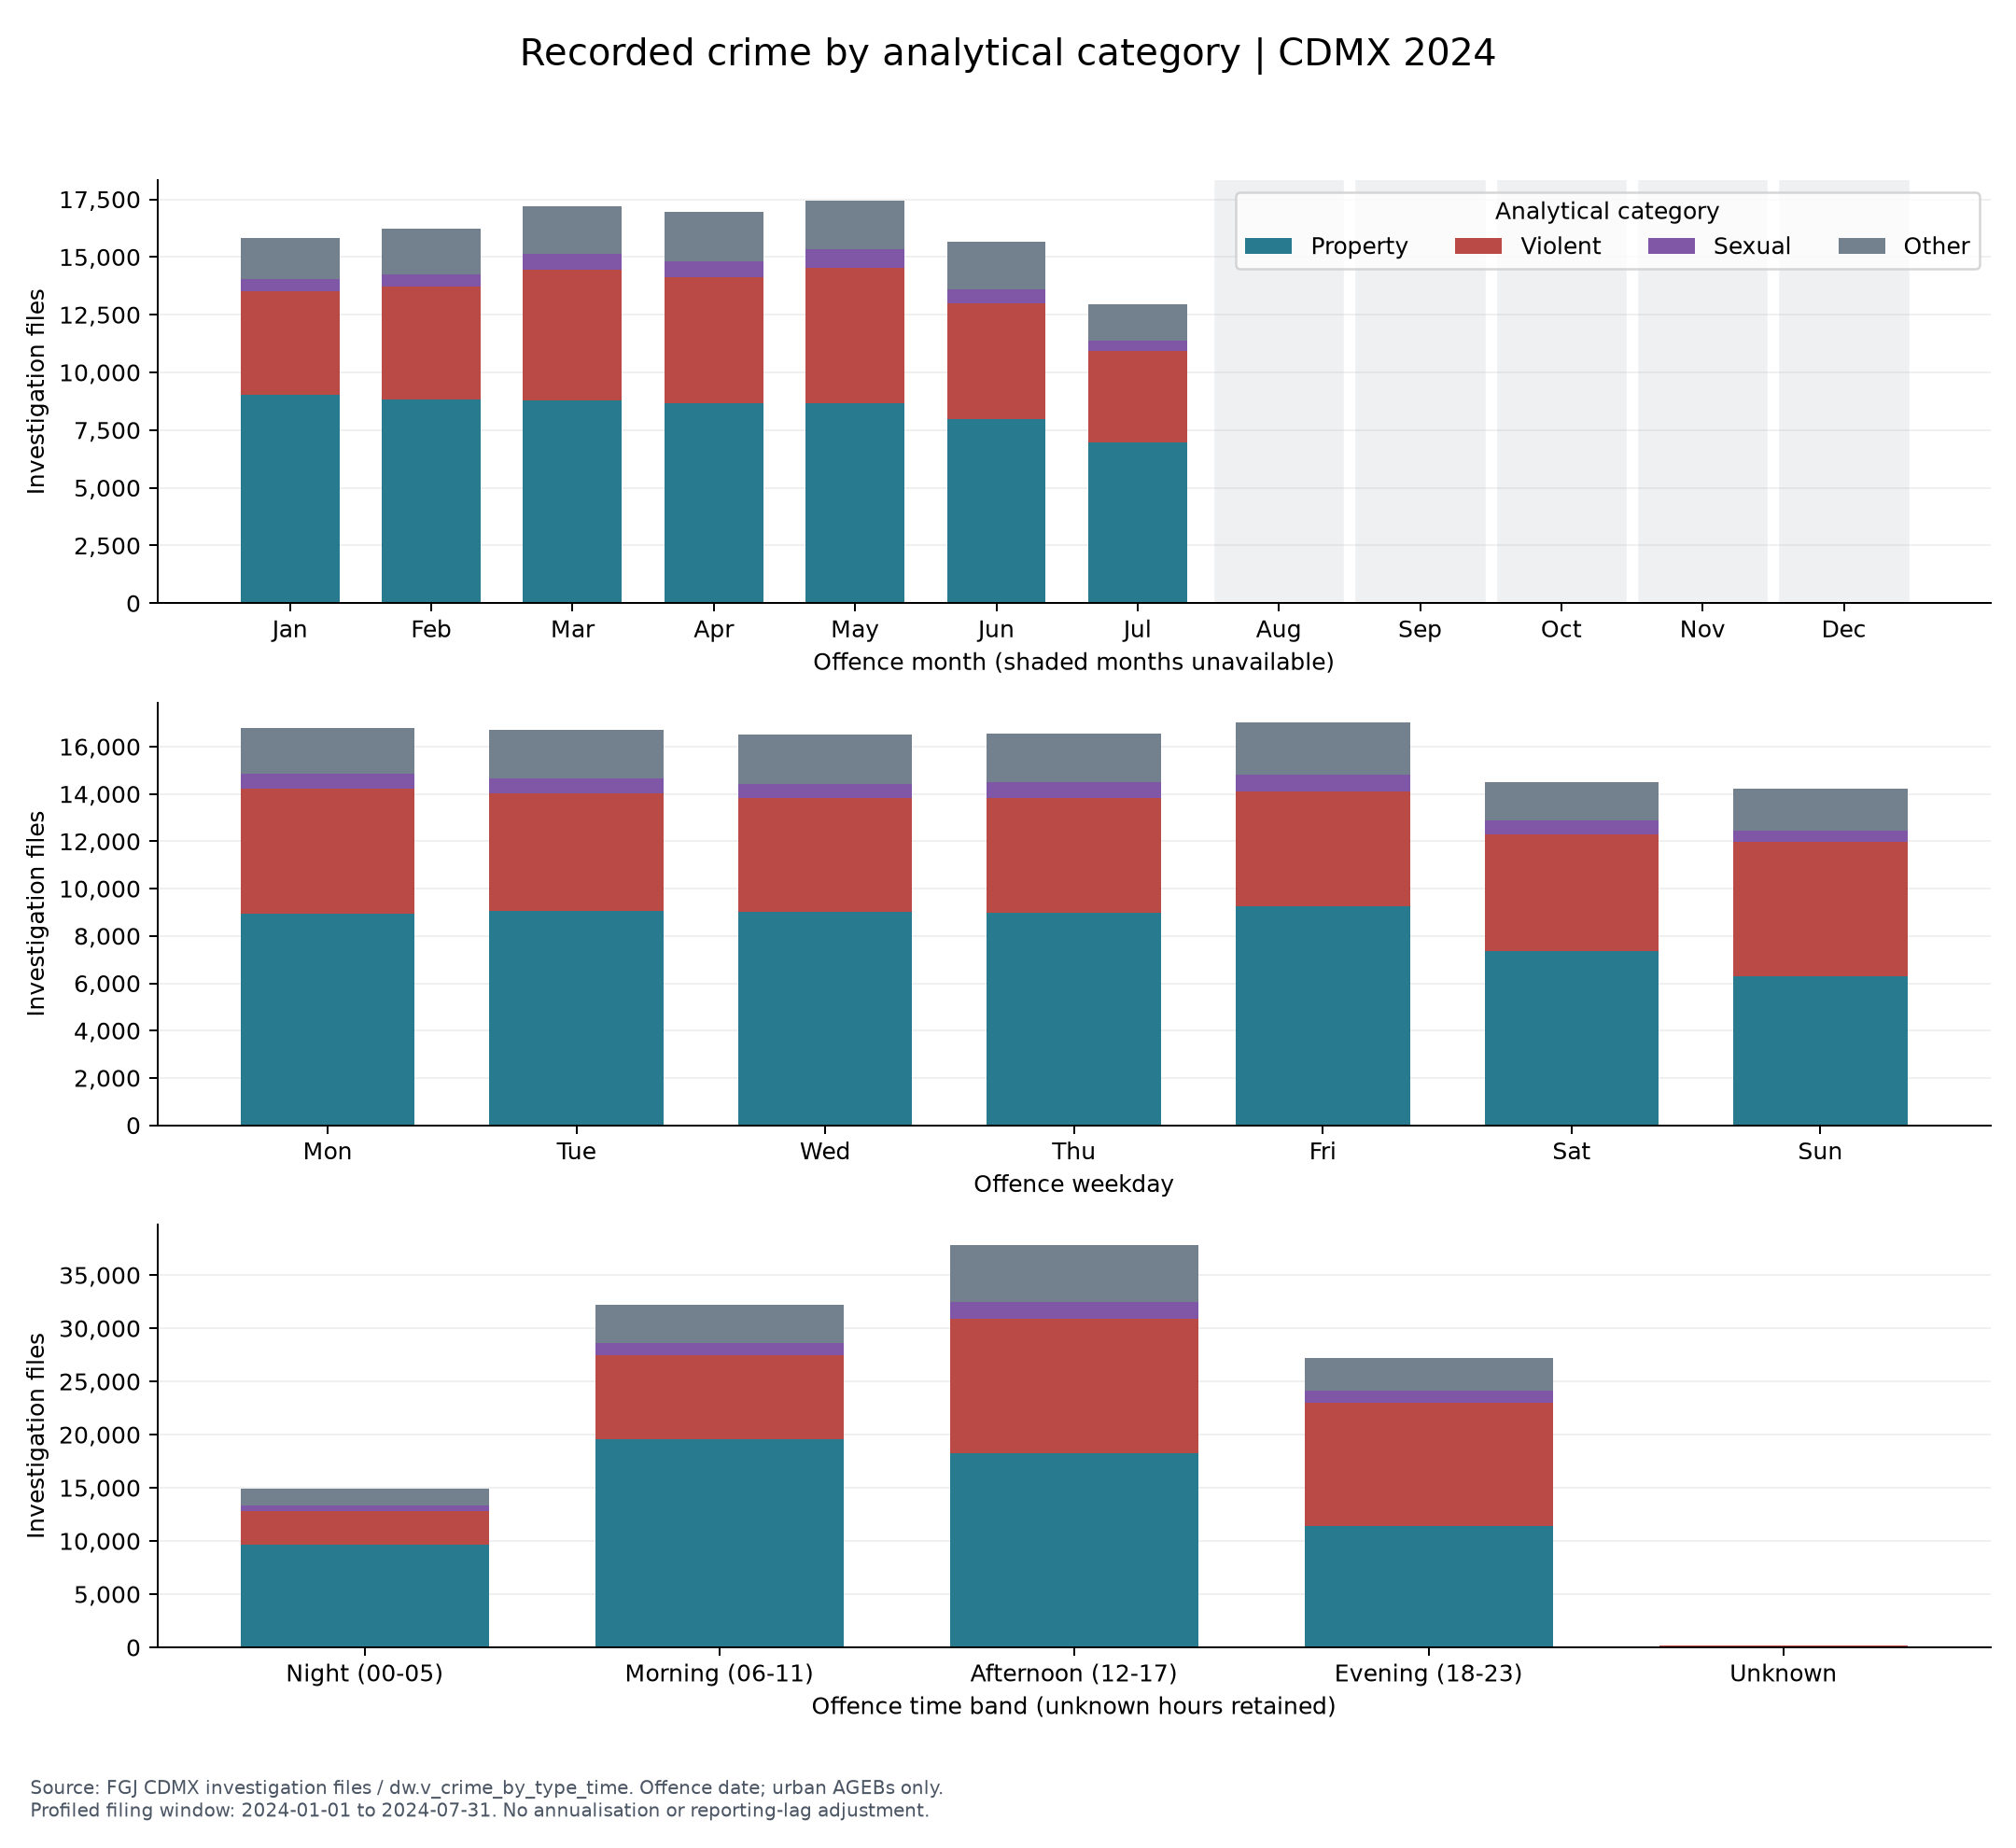
\includegraphics[width=\columnwidth]{crime_temporal_patterns.png}}
\caption{Investigation files by offence month, weekday and time band (112,285 files). July is partial; August--December are unavailable.}
\label{fig:time}
\end{figure}

\section{Limitations and Interpretation Cautions}

\textbf{Temporal mismatch.} Census 2020, FGJ January--July 2024 and DENUE 05/2026 are not simultaneous. A business observed in 2026 did not necessarily exist when a 2024 offence occurred. Seven months of crime data cannot establish annual seasonality. Counts are not annualised, and July is right-censored by the filing cutoff.

\textbf{Measurement.} Investigation files measure reported and recorded events, not all crimes or victims. Missing coordinates and the strict \texttt{within} rule remove 6.2\% of eligible files, possibly unevenly across space. Resident denominators omit commuters and visitors, and small populations inflate rates.

\textbf{Spatial inference.} Each LISA label is a separate test without multiple-comparison control. Permutation p-values do not preserve the autocorrelation of the other variable, and correlation p-values ignore spatial dependence. Results depend on the AGEB boundaries and scale (MAUP) \cite{openshaw1984}, and area-level associations do not describe individual behaviour (ecological fallacy). None of the associations reported here establishes causation.

\section{Conclusion}

The urban AGEB lets three independent official sources share a single geographic key without interpolating Census counts. A warehouse that keeps facts at their finest grain and computes every indicator in views makes each result reproducible from one command. In Mexico City, economic activity and recorded crime are both concentrated in the centre and spatially autocorrelated. Whether the centre stands out depends on whether crime is measured per resident or per establishment. Future work should add daytime-population denominators, a full year of crime data and spatial regression models that control for the dependence documented here.

\begin{thebibliography}{99}

\bibitem{inegi_census}
INEGI, ``Censo de Poblaci\'on y Vivienda 2020: principales resultados por AGEB y manzana urbana, Ciudad de M\'exico,'' Instituto Nacional de Estad\'istica y Geograf\'ia, 2021. [Online]. Available: \url{https://www.inegi.org.mx/programas/ccpv/2020/}

\bibitem{inegi_denue}
INEGI, ``Directorio Estad\'istico Nacional de Unidades Econ\'omicas (DENUE), Ciudad de M\'exico,'' Instituto Nacional de Estad\'istica y Geograf\'ia, May 2026. [Online]. Available: \url{https://www.inegi.org.mx/app/mapa/denue/}

\bibitem{inegi_mg}
INEGI, ``Marco Geoestad\'istico 2020, Ciudad de M\'exico,'' Instituto Nacional de Estad\'istica y Geograf\'ia, 2020. [Online]. Available: \url{https://www.inegi.org.mx/temas/mg/}

\bibitem{fgj}
Fiscal\'ia General de Justicia de la Ciudad de M\'exico, ``Carpetas de investigaci\'on FGJ de la Ciudad de M\'exico, 2024,'' Portal de Datos Abiertos CDMX, CC-BY-4.0. [Online]. Available: \url{https://datos.cdmx.gob.mx/}

\bibitem{moran1950}
P.~A.~P. Moran, ``Notes on continuous stochastic phenomena,'' \emph{Biometrika}, vol.~37, no.~1/2, pp.~17--23, 1950.

\bibitem{anselin1995}
L.~Anselin, ``Local indicators of spatial association---LISA,'' \emph{Geographical Analysis}, vol.~27, no.~2, pp.~93--115, 1995.

\bibitem{rey2007pysal}
S.~J. Rey and L.~Anselin, ``PySAL: A Python library of spatial analytical methods,'' \emph{The Review of Regional Studies}, vol.~37, no.~1, pp.~5--27, 2007.

\bibitem{benjamini1995}
Y.~Benjamini and Y.~Hochberg, ``Controlling the false discovery rate: A practical and powerful approach to multiple testing,'' \emph{Journal of the Royal Statistical Society: Series B}, vol.~57, no.~1, pp.~289--300, 1995.

\bibitem{pearson1897}
K.~Pearson, ``Mathematical contributions to the theory of evolution.---On a form of spurious correlation which may arise when indices are used in the measurement of organs,'' \emph{Proceedings of the Royal Society of London}, vol.~60, pp.~489--498, 1897.

\bibitem{openshaw1984}
S.~Openshaw, \emph{The Modifiable Areal Unit Problem}, ser. Concepts and Techniques in Modern Geography, no.~38. Norwich, U.K.: Geo Books, 1984.

\end{thebibliography}

\end{document}
